
\chapter{Approach}
\label{sec:approach}

This chapter gives a comprehensive description of the development of an Entity-based Sentiment Classifier for social media analysis, which is the ultimate result of this thesis. This approach relies on natural language processing (NLP) methods and machine learning (ML) tools to achieve a highly accurate sentiment classification. 

The following section presents the architecture and process pipeline of the entity-based sentiment classifier. Moreover, following sections provide an in depth description of the architecture's components.

\section{Architecture}

The architecture composition of the entity-based classifier is represented as a pipeline of processes. Each process is essential for the correct operation of the classifier, which is the following: 

\begin{enumerate}
\itemsep0em 

\item \textbf{Entity identification}

\item \textbf{Tokenization}

\item \textbf{Normalization}

\item \textbf{POS-Tagging}

\item \textbf{Feature Vector Generation}
\subitem - Document-based features
\subitem - Entity-based features

\item \textbf{Support Vector Machine}

\end{enumerate}

\begin{figure}
    \centering
    \caption{Processing pipeline and architecture}
    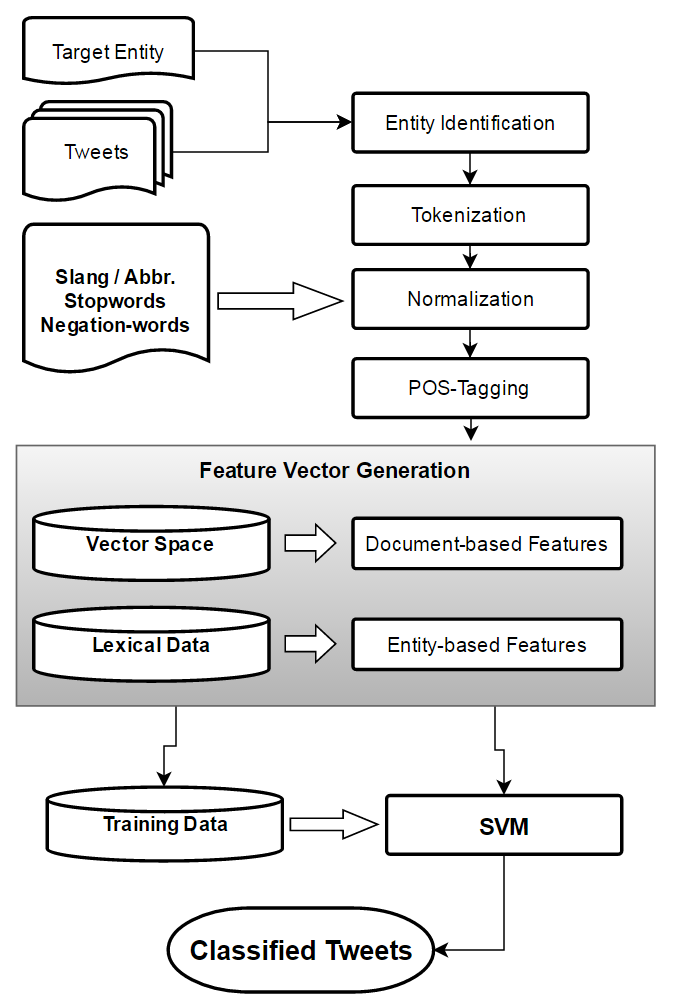
\includegraphics[width=\linewidth]{05_architecture}
    \label{fig5:architecture}
\end{figure}

\autoref{fig5:architecture} illustrates aforementioned components and processes. The pipeline starts with two input elements provided by the user or system which the classifier is integrated to. The required input data are the following:

\begin{itemize}
\itemsep0em 

\item \textbf{Tweet:} are microblogging-posts shared on the social media network Twitter. Tweets have a restriction of 140 characters and may contain URLs, mentions, hashtags or multimedia content. The classifier proposed in this thesis should be able to process every word or phrase contained in tweets in order to yield an accurate sentiment classification. For this task, specialized natural language processing methods are necessary.

\item \textbf{Target Entity:} The target entity refers to a query term (usually a company, product or person) which the classifier takes as an input in order to find the opinion expressed towards it. Therefore, given target entity must be present in the tweet. 

\end{itemize}

\begin{figure}[H]
    \centering
    \caption{Simplified entity-based sentiment classifier workflow}
    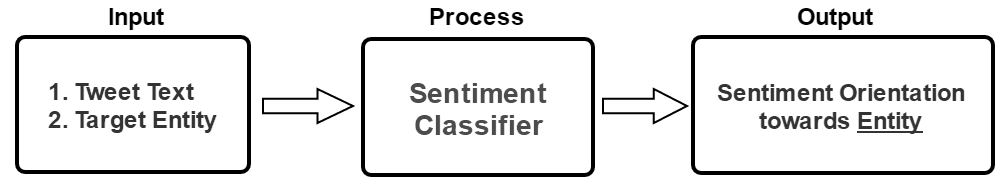
\includegraphics[width=\linewidth]{06_input_output}
    \label{fig6:input_output}
\end{figure}

\autoref{fig6:input_output} shows a simplified workflow of the entity-based sentiment classifier developed in this thesis. Notice that the input of the classifier is a 2-tuple (two elements list) composed by a tweet and a target entity. The output produced by the classifier is a three-class sentiment classification (positive, negative or neutral) which represents the opinion expressed in the tweet towards given target entity. Furthermore, continuing with the explanation of \autoref{fig5:architecture}, the first processing step in proposed system is called Entity Identification which will determine the presence of other entities (besides the target one) in the tweets. Then, the Tokenization step proceeds to remove unnecessary tokens (terms or words) or replace them with predefined placeholders. The workflow continues with a normalization process which is responsible for most of the linguistic processing in input tweets. After obtaining a normalized data, a POS-Tagger assigns part-of-speech labels to each token and sends them to the Feature Vector Generator. The Feature Vector Generator proceeds to extract document and entity level feature vectors to finally feed the support vector machine. The following sections will describe how each of these processes work.   

\pagebreak

\section{Entity Identification}

Entity identification, also known as Named-entity recognition (NER), is an information retrieval task that intends to label tokens of a given text into pre-defined categories such as companies, persons, locations, etc. The proposed approach requires the identification of entities in tweets to isolate contextual sentiments expressed towards the target entity. Therefore, opinions expressed towards non-target entities are not considered for sentiment classification. In following sections the entity contextual separation process is explained. 

\begin{figure}[H]
    \centering
    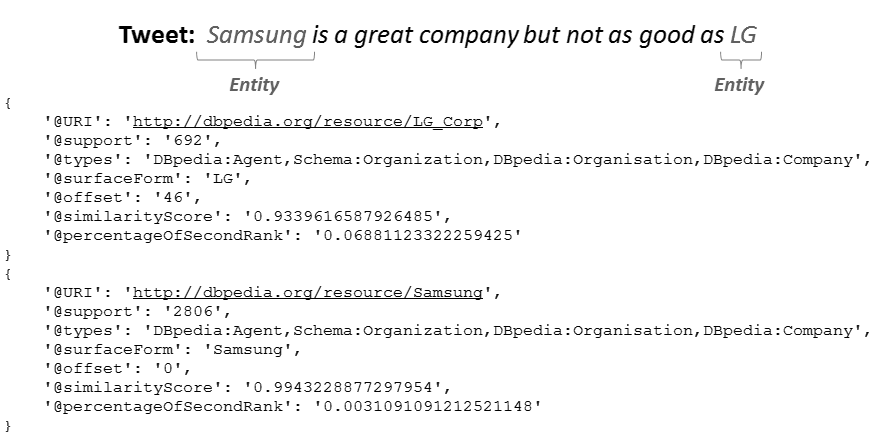
\includegraphics[width=\linewidth]{07_dbpedia_spotlight}
    \caption{DBPedia Spotlight annotation example}
    \label{fig7:dbpedia_spotlight}
\end{figure}

Proposed sentiment classification approach uses DBpedia Spotlight service in order to carry the entity identification task. This service annotates DBpedia\footnote{\url{http:wiki.dbpedia.org}} resources contained in the tweets, generating a list of contained entities. \autoref{fig7:dbpedia_spotlight} presents an example text annotated by Dbpedia Spotlight service which in this case provides meta-data about two identified DBpedia resources: \textit{Samsung} and \textit{LG}. Although the service returns information about entities such as \textit{type} and \textit{DBPedia URI}, proposed classifier only considers the identification of existing entities in given text ignoring the rest of the information. Further usage of DBpedia Spotlight service might be explored for future works and enhancements. Finally, a list of extracted entities is forwarded to the Tokenizer module which is explained in next section. 

\pagebreak

\section{Tokenization}

The Tokenization process is responsible for splitting input tweet text (string) into tokens (word or terms) and organize those tokens into their respective sentences. The Tokenizer (module in charge of this process) uses natural language processing methods and logistic rules such as regular expressions to trim the text. 

\begin{figure}[H]
    \centering
    \caption{Tokenization workflow}
    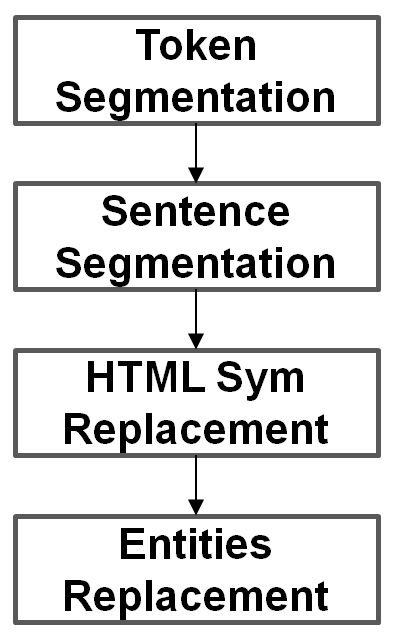
\includegraphics[width=6cm,height=9cm,keepaspectratio]{08_tokenization}
    \label{fig8:tokenization}
\end{figure}

In \autoref{fig8:tokenization} the Tokenization process workflow is represented. Starting with the \textit{token segmentation}, words contained in tweets are separated to each other based in the presence of white spaces. Then, a regular expressions algorithm checks each of those tokens for sentence stop punctuations such as exclamation points, question marks and full stops. This sentence segmentation step is necessary for the entity-based feature vector generation process since the sentiment relevance of sentences is associated with the presence of entity tokens. Finally, HTML symbols (e.g. \&amp, \&quot, etc) are replaced by their substituted values (some emoticons are made by this symbols) followed by the replacement of identified entities with respective placeholder. The replacement process of entities reduces the sparsity of future generation of vector space model. \autoref{tab:tokenizer_example} shows an example of a tokenized tweet where tokens are arranged into sentences and entities are replaced by their respective placeholders (\textit{TargetEntity and OtherEntity}).

\begin{table}[H]
\centering
\caption{Tokenized tweet example}
\label{tab:tokenizer_example}
\begin{tabular}{c|l}
{\color[HTML]{000000} \textbf{\begin{tabular}[c]{@{}c@{}}Target\\ Entity\end{tabular}}} & {\color[HTML]{000000} (1) Google}                                                                                                                    \\ \hline
\textbf{\begin{tabular}[c]{@{}c@{}}Other\\ Entities\end{tabular}}                       & (1) Nexus                                                                                                                                            \\ \hline
{\color[HTML]{000000} \textbf{Tweet}}                                                   & {\color[HTML]{000000} Thanks google!! Just got my new Nexus \&lt;3}                                                                             \\ \hline
{\color[HTML]{000000} \textbf{Result Tokens}}                                            & {\color[HTML]{000000} \begin{tabular}[c]{@{}l@{}}(1) \{Thanks, TargetEntity!!\}\\ (2) \{Just, got, my, new, OtherEntity, \textless3\}\end{tabular}}
\end{tabular}
\end{table}


\section{Normalization}
 \label{sec:normalization}

Executed by a preprocessor module, the normalization step does most of the linguistic processing required for generation of feature vectors. Normalization of data involves the correction, removal and replacement of tokens yield by the tokenization process.  While some Twitter features like \textit{@mentions} and \textit{URLs} are weightless in a sentiment context, \textit{\#hashtags} actually might contain sentiment value which is necessary for a final classification. The Normalization process is composed of five processing steps, these are represented in \autoref{fig9:normalization}. 

\begin{figure}[H]
    \centering
    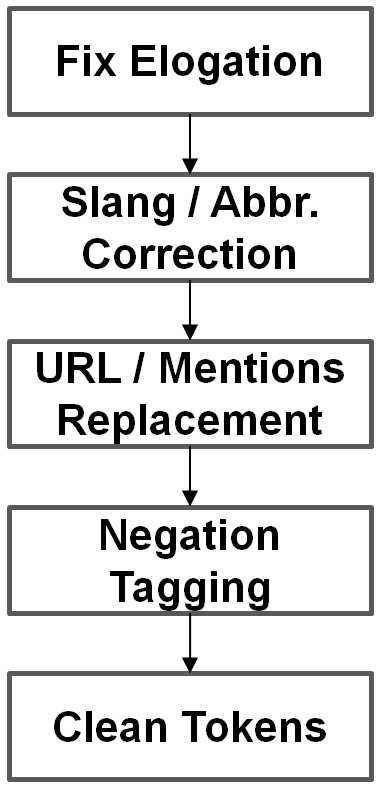
\includegraphics[width=7cm,height=10cm,keepaspectratio]{09_normalization}
    \caption{Normalization workflow}
    \label{fig9:normalization}
\end{figure}

\begin{itemize}
\itemsep0em 

\item \textbf{Fix Elongation}: tokens that contain more than two repeated letters are fixed, leaving only two of these letter. For example, the word: \textit{"loooove!"} would be replaced by \textit{"loove!"}. This process contributes with the effectiveness of the classifier because despite the fact that resulting fixed words might not necessary be the correct ones (originals), most lexicons consider two-letter elongated versions of terms.   

\item \textbf{Slang / Abbr. Correction}: presence of slang words and abbreviations are very common in microblogging sites such a Twitter. Therefore, to enhance the effectiveness of the lexicon features, these tokens are substituted by their correct forms. For example, the slang word \textit{"w8"} is replaced by \textit{"wait"} and \textit{"u"} replaced by \textit{"you"}. 

\item \textbf{URLs / Mentions Replacement:} in some cases URLs or user names (@mentions) are relevant for opinion extraction. The values by them self are ignored, but the fact that there are references to URLs and users might be useful. Hence, URLs and mentions are replaced by the placeholders \textit{"someURL"} and \textit{"someUser"} respectively.

\item \textbf{Negation Tagging}: negation words such as \textit{"not"} or \textit{"never"} can modify the sentiment orientation of a sentence. e.g. "I love you" is an obvious positive sentence, but "I do not love you" is considered negative. Therefore, to deal with this situation, a negation tagging "\_NEG" must be appended to tokens located between a negation word and the end of sentence. The sentiment of negated tokens will be shifted in the features generation stage of this classifier.  

\item \textbf{Clean Tokens}: As the final step in the normalization process, a removal of unnecessary tokens must be done. Stopwords like \textit{"you", "my" or "the"} do not represent any sentiment value, consequently, those are removed. Also, tokens with no letters (excluding emoticons) are ignored for further processing. 

\end{itemize}

\begin{table}[H]
\centering
\caption{Normalization example}
\label{tab:normalization_example}
\begin{tabular}{l|l}
\multicolumn{1}{c|}{{\color[HTML]{000000} \textbf{Tokens}}}                                                                      & \multicolumn{1}{c}{{\color[HTML]{000000} \textbf{Normalization Result}}}                                                                  \\ \hline
{\color[HTML]{000000} \begin{tabular}[c]{@{}l@{}}(1)\{not, their, best, !\}\\ (2)\{ http://t.co, @Muse, \#LiveMuse\}\end{tabular}} & {\color[HTML]{000000} \begin{tabular}[c]{@{}l@{}}(1)\{not, their\_NEG, best\_NEG, !\}\\ (2)\{ someURL, someUser, \#LiveMuse\}\end{tabular}}
\end{tabular}
\end{table}

\autoref{tab:normalization_example} presents an example of how the normalization process works, in this case two sentences are normalized. The first one shows the negation tagging of tokens \textit{"their" and "best!"} because they are positioned after the negation word \textit{"not"}. On the second sentence, an example of token replacements is shown.

\section{POS Tagging}

POS tagging consists on labeling normalized tweet tokens with their respective part-of-speech (POS) values. There are many POS tagging technologies but only a few of them are design to perform Twitter-specialized POS analysis. The solution proposed in this master's thesis uses Twitter ARK POS Tagger which is a java-based part-of-speech tagger for English data and it is tailored made for Twitter posts. ARK POS Tagger was developed by a group of researchers from Carnegie Mellon University\footnote{\url{http://www.cmu.edu/}}, they manually annotated 1,827 tweets with POS tags and developed a specialized POS tagset for tweets. ARK POS Tagger reports nearing 90\% accuracy~\cite{gimpel2011part} making it one of the most effective solutions available.  

\autoref{fig10:pos_table} shows the ARK POS tagset with examples for each POS tag. The most relevant POS tags for sentiment classification are adjectives \textit{(tag:A)} and nouns \textit{(tag:N)} which usually express some degree of sentiment. For this reason, sentiment lexicons like \textit{SentiWordNet} and \textit{AFINN} are mostly composed by nouns and adjectives. However, hashtags \textit{(tag:\#)} in tweets may also contribute significantly with the extraction of sentiment expressions. For example, the hashtag \textit{\#BeautifulDay} clearly has a positive connotation. 

\begin{table}[H]
\centering
\caption{ARK POS Tagging example over normalized tokens}
\label{tab:pos_tagging_example}
\begin{tabular}{l|l}
\multicolumn{1}{c|}{{\color[HTML]{000000} \textbf{Normalized Tokens}}}                                                                      & \multicolumn{1}{c}{{\color[HTML]{000000} \textbf{POS Tagging}}}                                                                                      \\ \hline
{\color[HTML]{000000} \begin{tabular}[c]{@{}l@{}}(1)\{not, their\_NEG, best\_NEG\}\\ (2)\{ someURL, someUser, \#Live\}\end{tabular}} & {\color[HTML]{000000} \begin{tabular}[c]{@{}l@{}}\{R/not, O/their\_NEG, A/best\_NEG\}\\ \{ someURL, someUser, \#/\#Live\}\end{tabular}}
\end{tabular}
\end{table}

\autoref{tab:pos_tagging_example} shows how the POS tagging process works. In this example, the normalized tokens \textit{not, their\_NEG, best\_NEG and \#Live} are replaced by \textit{R/not, O/their\_NEG, A/best\_NEG and \#/\#Live} respectively. The symbol "/" is appended at the beginning of each token, even if those tokens are already tagged as negated (\_NEG). Additionally, tokens already identified on previews steps are ignored by the POS tagger. e.g. "@mentions", "URLs" and "punctuation symbols". This is the final processing step before starting the feature vector generation. Following sections will explain how these tokens are transformed into vectors that will represent  key component of proposed entity-based sentiment classifier. 

\begin{figure}[H]
    \centering
    \caption[ARK POS Tagset table with examples]{ARK POS Tagset table with examples ~\cite{gimpel2011part}}
    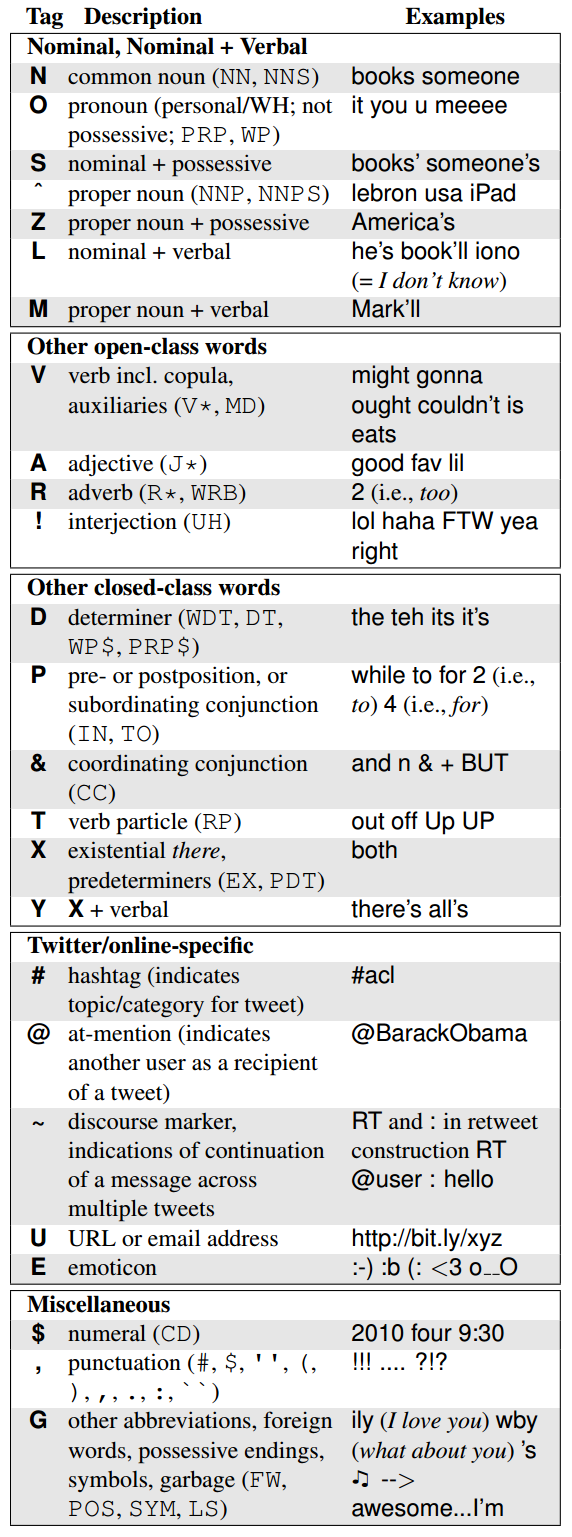
\includegraphics[width=15cm,height=23cm,keepaspectratio]{10_pos_table}
    \label{fig10:pos_table}
\end{figure}

\section{Feature Vector Generation}

The feature vector generation process is arguably the most important component in any sentiment classifier. A Support Vector Machine (SVM) based classifier like the one presented and implemented for this master's thesis, depends highly on the quality of features extracted from the raw data (tweets in this case). Therefore, in order to achieve a highly accurate classification, the production of feature vectors most be done with precision. The feature generation module is responsible for the extraction of numerical values from the already normalized and tagged tokens, the way these values are generated depends on the type of features required. Hence, this section explores two types of features: document-based and entity-based features. The sentiment classifier developed in this master's thesis uses both types of feature extraction, classifying tweets not only on a document-level like most sentiment classifiers but also on an entity-level which is the final goal of this project.   

\subsection{Document-based features generation}

Document-based features are those extracted from document-level data. This means that every single normalized-tagged token obtained from the input tweets is relevant and considered for the generation of vectors. As a result, each tweet is represented as a feature vector made up of the following set of features: binary bag-of-words (unigrams), POS tags, linguistic features.

\subsubsection{Binary bag-of-words}

Bag-of-words approach is used in natural language processing to represent training data (documents) as a set of word. This set of words is called vector space and will be made of every token existing in the training data. Then, new documents to be classified must be evaluated with aforementioned vector space to generate a vector representation of this new entry. The n-gram approach is a common way of categorizing words from documents and validate their presence in the vector space. In this master's thesis approach, unigrams were used to generate a vector space of the training data (tweets). There are many ways of representing unigrams in feature vectors but the binary approach was the selected method to be used in this project. Binary approach provides its simplicity and performance speed without scarifying quality. Binary bag-of-words also known as boolean term frequency, consists on representing terms contained in documents as 1s or 0s, where 1 means that the term is present and 0 thath it is absent. \autoref{tab:binary_bagofwords} shows an example of how a generated binary bag-of-words based on unigrams looks like.

\begin{table}[H]
\centering
\caption{Binary bag-of-words representation of a tweet}
\label{tab:binary_bagofwords}
\begin{tabular}{l|l}
\multicolumn{1}{c|}{{\color[HTML]{000000} \textbf{Tweets}}} & \multicolumn{1}{c}{{\color[HTML]{000000} \textbf{Binary Bag-of-words}}} \\ \hline
{\color[HTML]{000000} happy birthday friend! :)}            & {\color[HTML]{000000} \{1,1,1,1,0,0,0\}}                                \\ \hline
always be happy ;)                                          & \{1,0,0,0,1,1,1\}                                                      
\end{tabular}
\end{table}

\subsubsection{POS Tags}

The feature vector generated from part-of-speech (POS) Tags, consists on the number of \textit{verbs, adverbs, adjectives and nouns} contained in tweets. Inspired by Saif et al.~\cite{MohammadKZ2013}, these four POS tags are proved to be the most relevant for sentiment classification. The addition of more POS tags to the feature generation process might have a negative impact on the classification accuracy. In \autoref{tab:pos_vector} an example of POS tag features is shown, the order of POS tags for the creation of vectors is the following:  \textit{(1)noun -> (2)adjective -> (3)adverb -> (4)verb}

\begin{table}[H]
\centering
\caption{POS Tag feature vector example}
\label{tab:pos_vector}
\begin{tabular}{l|l}
\multicolumn{1}{c|}{{\color[HTML]{000000} \textbf{Tweets}}} & \multicolumn{1}{c}{{\color[HTML]{000000} \textbf{POS Tags}}} \\ \hline
{\color[HTML]{000000} happy birthday friend! :)}            & {\color[HTML]{000000} \{2,1,0,0\}}                           \\ \hline
always be happy ;)                                          & \{0,1,1,1\}                                                 
\end{tabular}
\end{table}

\subsubsection{Linguistic features}

Linguistic features are a set of elements extracted from tweets and represented as count numbers on feature vectors.  The Linguistic features consists of the following eight
elements:

\begin{enumerate}
\itemsep0em 

\item \textbf{all-caps}: the number of words with all characters in upper case.

\item \textbf{hashtags}: the number of hashtags present in the tweet.

\item \textbf{elongated words}: the number of elongated words. e.g. \textit{loooove!}

\item \textbf{negation context}: the number of negation contexts.

\item \textbf{punctuation}: count of contiguous sequences of question marks, exclamation marks, and both exclamation and question marks. e.g. \textit{!!!, ???, !!??}

\end{enumerate}

\subsection{Entity-based features generation}
\label{sec:feature_generation}

Entity-based features unlike document-based, are extracted from entity-level data. Entity-level data can be described as the context information of a target entity. The idea is to separate the contextual sentiment of every existing entity in a document (tweet in this case), then generate sentiment features only for the target entity ignoring non-target ones. Therefore, this subsection explains which entity-base features were used for the development of proposed entity-based classifier. 

\begin{figure}[H]
    \centering
    \caption{Entity-based features generation workflow}
    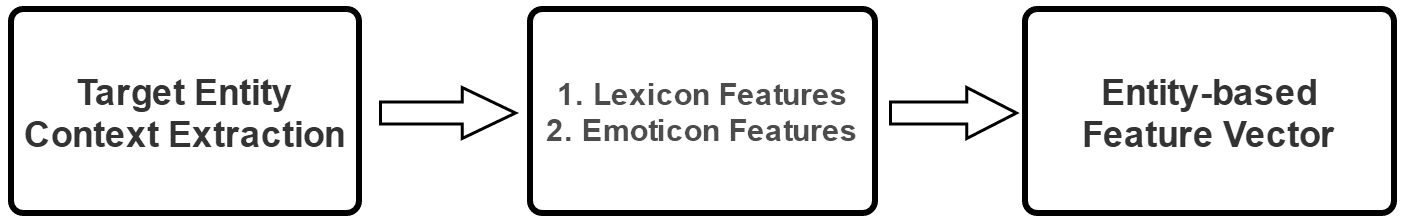
\includegraphics[width=\linewidth]{11_entity_based_features}
    \label{fig11:entity_based_features}
\end{figure}

\autoref{fig11:entity_based_features} illustrates the processing steps required for the generation of entity-based features, it starts with the identification of the target entity context. The following techniques were used in order to extract target contexts:

\begin{enumerate}
\itemsep0em 

\item \textbf{Sentence separation}: A tweet may contain many entities but only the target entity and its context should be considered for entity-level feature generation. Therefore, each sentence in a given tweet is evaluated for entity presence and only those that fulfil the following rules are considered: (1) sentence with target entity (2) sentence with no entities that is in the neighborhood of a target entity sentence. For a better illustration of this concept,  \autoref{fig12:feature_sentence_context} shows how the identification of relevant context is done in a tweet with two sentences, the first is relevant because it contains the target entity \textit{"Nexus 5X"} while the second sentence is ignored due to other entity presence (\textit{"Apple"}).  

\begin{figure}[H]
    \centering
    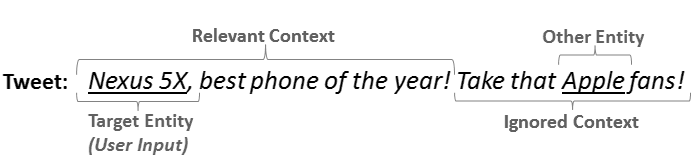
\includegraphics[width=\linewidth]{12_feature_sentence_context}
    \caption{Sentence separation context identification of tweet}
    \label{fig12:feature_sentence_context}
\end{figure}

\pagebreak

\item \textbf{"But" clause}: "But" clause context extraction method is similar to a sentence separation process. Sentences with "but" like clauses (“with the exception of”, “except that” and “except for”) are splinted using as separation point the position of these clauses. \autoref{fig13:but_clause_context} illustrates this idea, for this example only the content to the left side of the token "but" will be extracted an considered for sentiment evaluation. The remaining part of the sentence is irrelevant due to the presence of another entity (no-target).

\end{enumerate}

\begin{figure}[H]
    \centering
    \caption{But clause context extraction of tweet}
    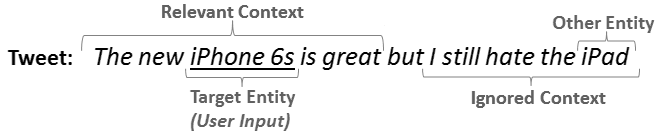
\includegraphics[width=\linewidth]{13_but_clause_context}
    \label{fig13:but_clause_context}
\end{figure}

\subsubsection{Lexicon Features}

After a successful extraction of sentiment contexts, lexical features can be generated from those contexts. Lexicon features are the heart of a sentimentt classifier and usually represent the most effective set of features.  Many different opinion lexicons can be used to represent the numerical sentiment values of tweets. Hence, the classifier presented in this master's thesis combines seven different state-of-the-art sentiment lexicons.  For each of these lexicons, the following set of features is calculated to generate a compelling sentiment feature vector~\cite{MohammadKZ2013}:

\begin{enumerate}
\itemsep0em 

\item \textbf{No. Tokens}: the number of sentiment tokens in the tweet.  These tokens are words with sentiment scores above or below zero in a lexicon.

\item  \textbf{Total Score}: total sentiment score calculated in tweet. 

\item \textbf{Max Score}: highest sentiment score obtained in the tweet.

\item \textbf{Last Token}: sentiment score of last token.

\end{enumerate}

When an entity context has negated tokens, sentiment scores for those tokes are inverted. The solutions presented in this project uses a combination of different lexicons, the quality of these lexicons is critical for the classifier. Therefore, the following state-of-the-art lexical resources were selected for this task:  

\pagebreak

\begin{itemize} 
\itemsep0em  

\item \textbf{MaxDiff}~\cite{kiritchenko2014sentiment}: It is a manually labeled lexicon developed by crowdsourcing and using the MaxDiff method. The lexicon contains 1,500 positive and negative words which are scored from -1 to 0 and 0 to 1.

\item \textbf{Bing Liu}~\cite{hu2004mining}~\cite{liu2005opinion}: Developed by Bing Liu, all terms of this lexicon are manually labeled. It contains 6.790 positive and negative words which are not scored.

\item  \textbf{AFINN}~\cite{nielsen2011new}: Manually labeled lexicon composed by 2.477 words, each word has a sentiment score in the range of -5 to 5. 

\item \textbf{SentiWordNet}~\cite{esuli2006sentiwordnet}: built over WordNet lexical database which contains ~150.000 words. This lexical resource assigns sentiment scores in a range of -1 to 1 with decimal values. Unlike BingLiu and AFINN lexicons, SentiWordNet scores are semi-automatically generated from manually labeled seed-words using  semi-supervised techniques. 

\item \textbf{MPQA}~\cite{wilson2005recognizing}: just like SentiWordNet, MPQA is a subjectivity lexicon created by using semi-supervised techniques. This lexical resource has 6.880 labeled words with no score intensities, only positive and negative.   

\item \textbf{NRC Hashtag / Sentiment140}~\cite{NRCJAIR14}: Developed by Mohammad Saif, both lexicons were generated fully automatically with distant supervision techniques. NRC Hashtag and Sentiment 140 lexicons contain 54,129 and 62,468 words respectively. Both represent the sentiment value of words with scores between -$\infty$ (most negative) to $\infty$ (most positive).


\end{itemize}

\begin{table}[H]
\centering
\caption{Lexical resources summary.}
\label{tab:lexical_resources}
\begin{tabular}{|l|c|c|}
\hline
\multicolumn{1}{|c|}{\textbf{Lexicon}} & \textbf{Score Range} & \textbf{No. Words} \\ \hline
MaxDiff Twitter                        & Real-values          & 1,500              \\ \hline
AFINN                                  & -5 to 5              & 2,477              \\ \hline
BingLiu                                & Pos / Neg            & 6,785              \\ \hline
SentiWordNet                           & -1 to 1              & 147,292            \\ \hline
MPQA                                   & Pos / Neg            & 6,886              \\ \hline
NRC Hashtag                            & Real-values          & 54,129             \\ \hline
Sentiment140                           & Real-values          & 62,468             \\ \hline
\end{tabular}
\end{table}

\pagebreak

\subsubsection{Emoticon Features}

The informal nature of tweets is characterized by the common usage of emoticons to express sentiment. Therefore, emoticons are also considered for the generation of feature vectors. Only those emoticons contained on the target-entity context are used to generate this features. The vector composition is fairly simple: \textit{No. of positive emojis (e.g. ":)", ":D", ";)" ) / No. of negative emojis (e.g. ":(", "D:")}.

In \autoref{tab:entity_vectors} an example of entity-based feature vectors is presented. Notice that there is only one emoticon in the example and it has positive value, hence the result vector is {1,0} (+1 positive, 0 negative). Similar rules apply to BingLiu lexicon features, two positive words in the tweet with no negative sentiments. 

\begin{table}[H]
\centering
\caption{Entity-based feature vectors example}
\label{tab:entity_vectors}
\begin{tabular}{l|l}
\multicolumn{1}{c|}{{\color[HTML]{000000} \textbf{Target-entity context tokens}}}                                         & \multicolumn{1}{c}{{\color[HTML]{000000} \textbf{Feature Vectors}}}                                     \\ \hline
{\color[HTML]{000000} \begin{tabular}[c]{@{}l@{}}\{my, TargetEntity, is, {\color[HTML]{036400}awesome}, \\ {\color[HTML]{036400}best}, day, ever, {\color[HTML]{036400}:D} \}\end{tabular}} & {\color[HTML]{000000} \begin{tabular}[c]{@{}l@{}}(BingLiu)\{2, 2, 1, 1\}\\ (Emoji)\{1,0\}\end{tabular}}
\end{tabular}
\end{table}

\section{Support Vector Machine}

This component represents the final stage of proposed sentiment classification solution. There are many supervised learning models such as Maximum Entropy, Naive Bayes and Neural Networks. However, Support Vector Machines (SVMs) have the potential to handle large feature spaces in a very efficient way~\cite{joachims1998text}. Hence, a SVM is used to deal with the large set of features generated from tweets and entities, the generation of this features is explained in \autoref{sec:feature_generation}. Like any other supervised learning model, SVMs require training data to function. This training data is represented as numerical feature vectors labeled with their respective class, the labeling process is usually done manually (by evaluators) but in some cases distant-supervision methods are used. The job of any SVM is to find a clear separation between training vectors and their classes, based on this learning process, the SVM is able to classify new document entries (tweets for this case). 

Proposed entity-based classifier uses a support vector machine (SVM) NodeJS module called \textit{Node-SVM} which is a port from the C++ SVM library \textit{LIBSVM}~\cite{chang2011libsvm}. This library is one of the most popular SVM solutions available for machine learning based classification and regression. To have a better understanding of implemented classifier, the parameters used to setup \textit{Node-SVM} are the following:

\begin{itemize} 
\itemsep0em  

\item \textbf{SVM Type:} C-Support Vector Classification (C\_SVC). n-class classification where n $>$ 2, allows multi-class classification (positive, negative and neutral).

\item  \textbf{Kernel}: Default Liner kernel is used.  

\item  \textbf{Normalization}: During SVM data pre-processing, mean normalization is required.  

\item  \textbf{Shrinking}: Usage of shrinking heuristics.  

\item  \textbf{Probability}: Disable the usage of probability estimates.  

\end{itemize}

\autoref{fig15:linear_svm} illustrates the linear form of a SVM which is a hyperplane that divides a set of positive data points (positive labeled tweets) from a set of negative data points. The separation distance between these two set is called \textit{maximum margin}. In linear SVMs, the maximum margin represents the maximum distance of the hyperplane to the positive and negative data points. 

\begin{figure}[H]
    \centering
    \caption[Illustration of a linear Support Vector Machine]{Illustration of a linear Support Vector Machine{~\cite{platt1998sequential}}}
    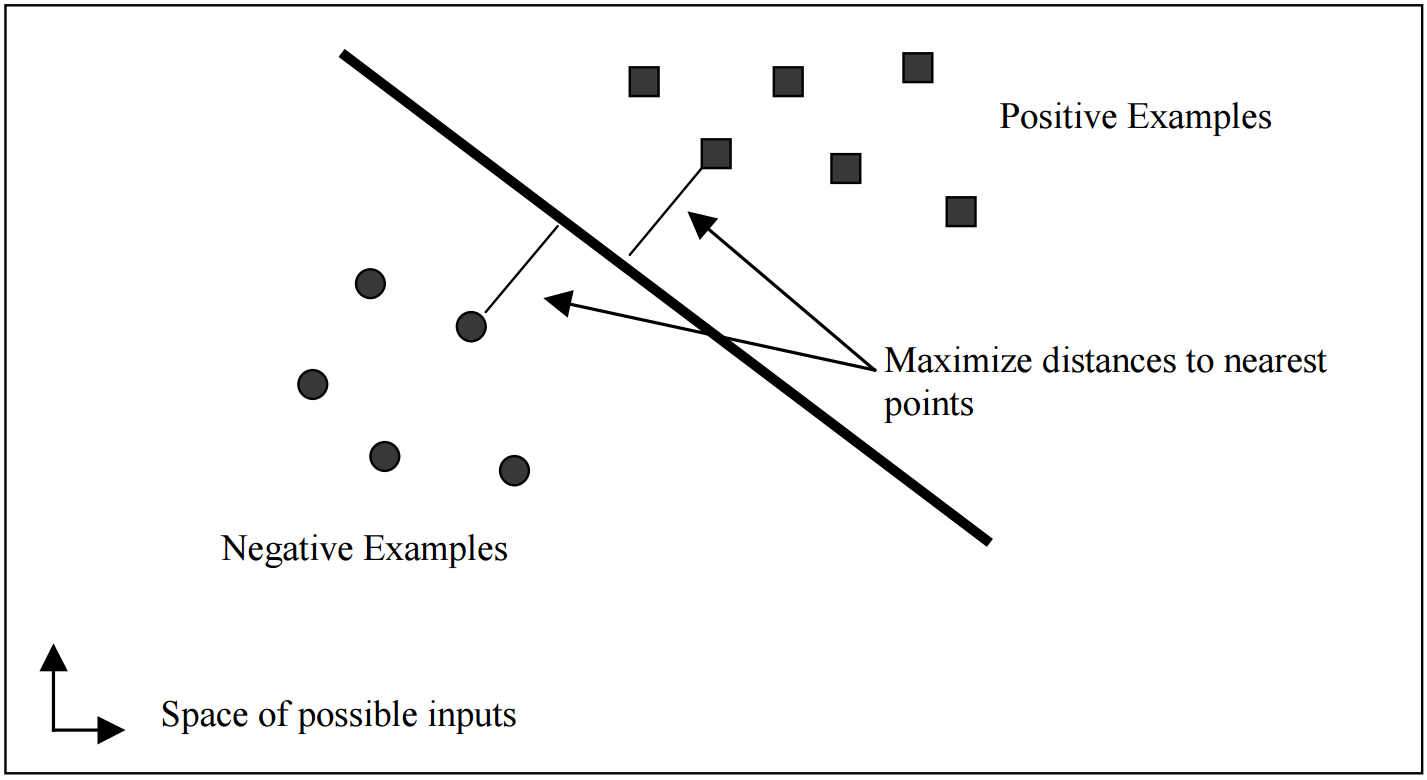
\includegraphics[width=\linewidth]{15_linear_svm}
    \label{fig15:linear_svm}
\end{figure}


\section{SentiTrack Integration}

For a full description of the SentiTrack system refer to \autoref{sec:sentitrack}. The integration process of the sentiment classifier developed in this master's thesis and the SentiTrack system was fairly simple since both platforms are fully developed with NodeJS (JavaScript) technologies. Therefore, in order to perform the integration, the proposed classifier was implemented as a NodeJS module using the JS package manager (npm) approach. \autoref{fig16:package_files} shows the package organization of implemented module (source code files), the name of the module is \textit{entity\_sentiment} which refers to the capabilities of implemented entity-based sentiment classifier. The following line of code is required to make use of the \textit{entity\_sentiment} module:

 \begin{displayquote}
var entitysentiment = require("entity\_sentiment");
\end{displayquote} 

This line will allow NodeJS classes to perform classification using proposed solution. In following \autoref{sec:evaluation} the quality and performance of developed classifier is tested and evaluated, then an analysis of result is presented. 

\begin{figure}[H]
    \centering
    \caption[Package files organization]{Package files organization}
    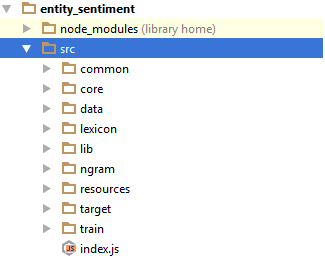
\includegraphics[width=9cm,height=13cm,keepaspectratio]{16_package_files}
    \label{fig16:package_files}
\end{figure}
